\section{Design of Architecture} \label{sec:overview}

Figure 2 shows our proposed architecture in KVM virtualization environment. 
It contains three main components: the Serviceguard, a tailored version 
of QEMU, and the \smr system \smrsystem. 
Only the primary VM advertises its presence on the network, so all network input come 
to the primary physical host. 
The Serviceguard is deployed on the virtual machine, and provides high availability 
of applications running on virtual machines. 

\begin{figure}[t]
% \vspace{.20in}
\centering
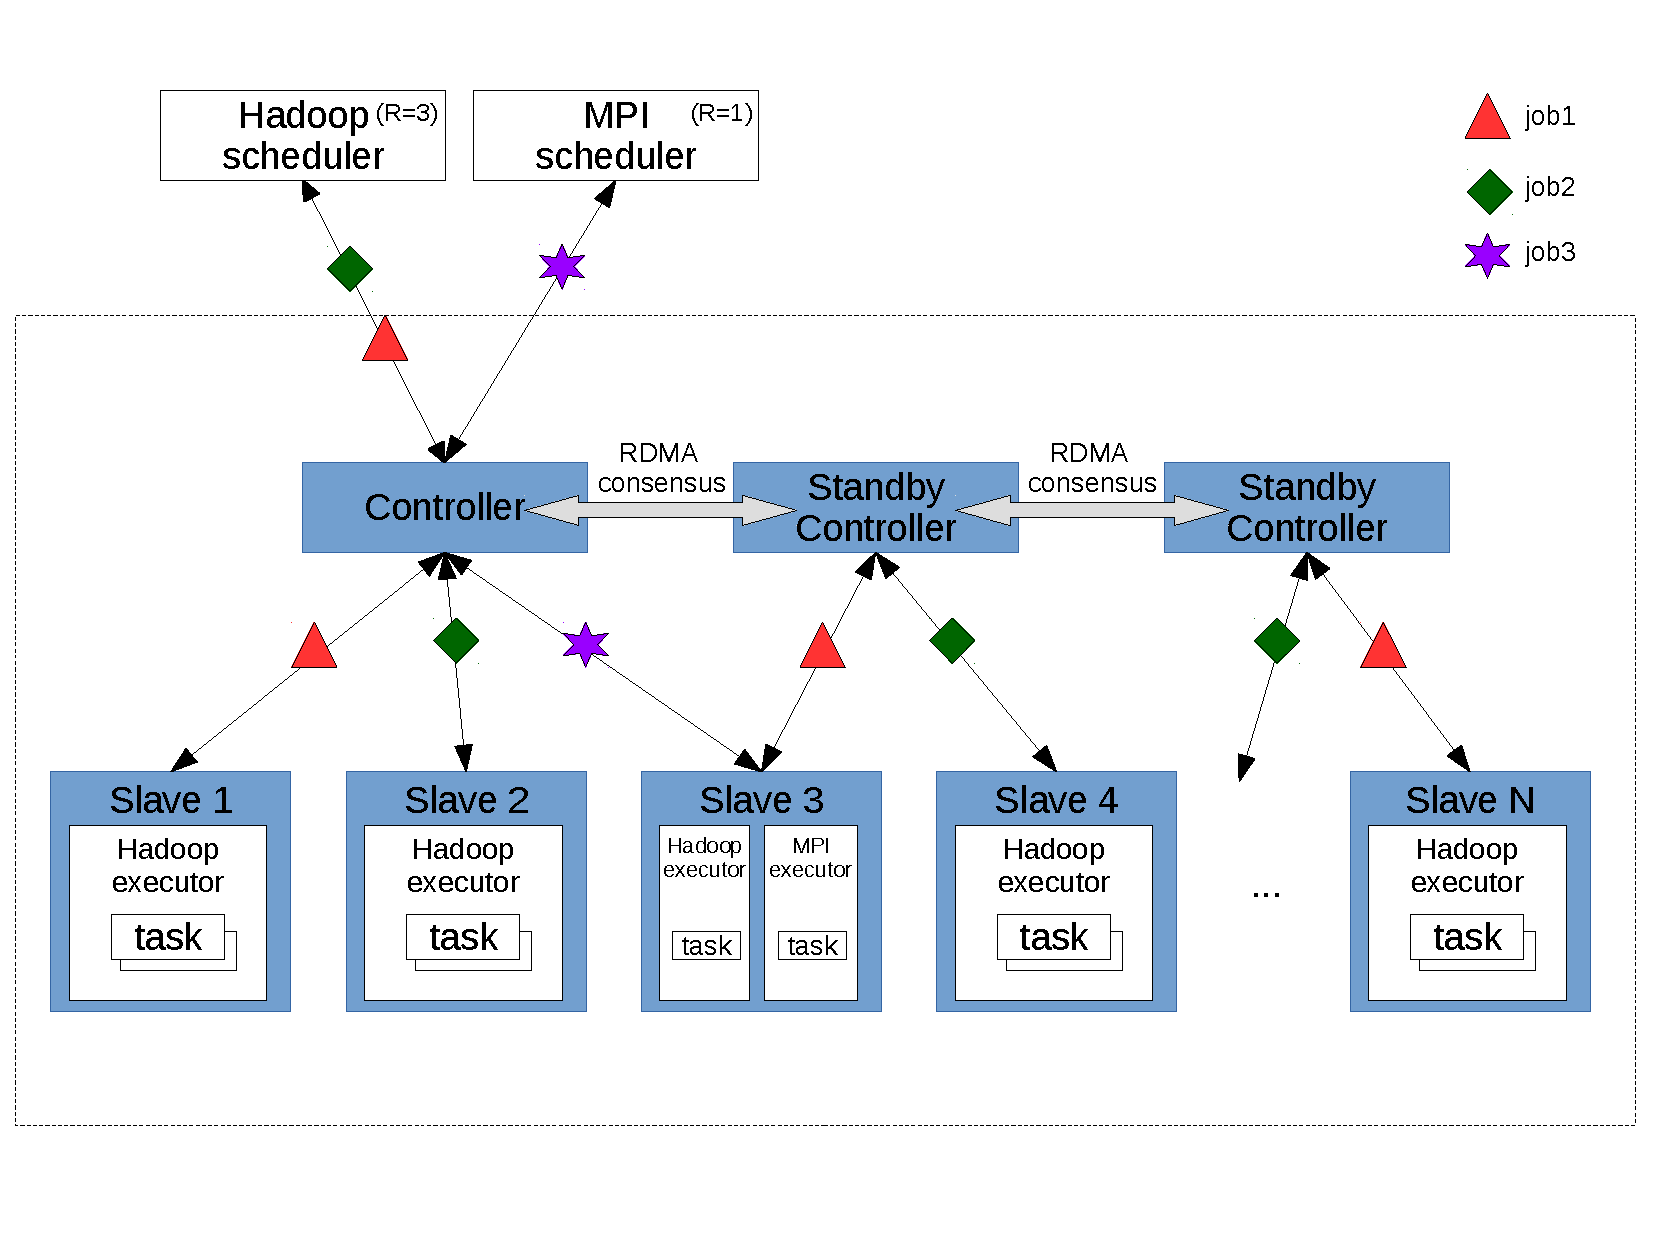
\includegraphics[width=.47\textwidth]{figures/arch}
\vspace{-.2in}
\caption{{\em Proposed architecture in KVM virtualization environment.} Key 
components are shaded (and in blue).} \label{fig:arc}
\vspace{.05in}
\end{figure}
